%\documentclass[handout]{beamer}
\documentclass{beamer}
\usepackage{amsmath}
\usepackage{stdpresent}
%\usepackage[margin=1in]{geometry}
\usepackage{tikz}
\usepackage{natbib}
\usepackage{booktabs}
\usepackage{verbatim}
\usepackage{tikz}
\usetikzlibrary{intersections,positioning}
\usetikzlibrary{matrix, calc}
\newcommand*{\hnode}[1]{\node[outer sep=0pt,anchor=base] (#1) {#1};} 
\usepackage[absolute,overlay]{textpos}
\usetikzlibrary{bayesnet}
\usepackage{tcolorbox}
\usepackage{subfigure}
\usepackage{stackengine}
\usepackage{vimacros}

%\usepackage{subcaption}
\usepackage[tikz]{bclogo}


\newcommand{\cblue}[1]{\textcolor{blue}{{#1}}}
\newcommand{\cred}[1]{\textcolor{red}{{#1}}}

\title[DGM4NLP]{Generative models of word representation}
\subtitle{DGM4NLP}

\def\W#1#2{\rnode{#1}{#2}\hfill}

\newcommand{\pointthis}[2]{
        \tikz[remember picture,baseline]{\node[anchor=base,inner sep=0,outer sep=0]%
        (#1) {\textbf{#1}};\node[overlay,rectangle callout,%
        callout relative pointer={(0.1cm,0.5cm)},fill=yellow!90] at ($(#1.north)+(-.5cm,-1cm)$) {#2};}%
        }%

\newcommand{\ack}[1]{\let\thefootnote\relax\footnote{\textcolor{gray}{#1}}}

\presetkeys{bclogo}{
ombre=true,
epBord=3,
couleur = blue!15!white,
couleurBord = red,
arrondi = 0.2,
logo=\bctrombone
}{}

\author[Rios]{Miguel Rios\\University of Amsterdam}
\date{\today}

% add page num
\expandafter\def\expandafter\insertshorttitle\expandafter{%
  \insertshorttitle\hfill%
  \insertframenumber\,/\,\inserttotalframenumber}

\begin{document}
\maketitlepage


\section{Word embeddings}

\frame{ \frametitle{Introduction}

\begin{textblock*}{\textwidth}(0.1\textwidth,0.25\textheight)
\center Discriminative embedding models\\ \textbf{word2vec} 
\end{textblock*}

\begin{textblock*}{\textwidth}(0.1\textwidth,0.4\textheight)
	\begin{small}
	\begin{center}
	%\only<1>{
	%\emph{\textcolor{blue}{In the event of a chemical spill,} \textcolor{blue}{most children know they should} {\bf evacuate} \textcolor{blue}{as advised by people in} \textcolor{blue}{charge.}}}
	%\only<2-4>{
	\emph{\textcolor{red}{In the event of a chemical spill,} \textcolor{blue}{most children know they should} {\bf evacuate} \textcolor{blue}{as advised by people in} \textcolor{red}{charge.}}
	%}
	%\only<5->{
	%\emph{\textcolor{red}{In the event of a chemical spill,} \textcolor{blue}{most children know they should} \pointthis{evacuate}{ambiguity} \textcolor{blue}{as advised by people in} \textcolor{red}{charge.}}}
	\end{center}
	\end{small}
	\end{textblock*}
	
	
	\begin{textblock*}{\textwidth}(0.2\textwidth,0.6\textheight)
	
	\only<1->{
	Place words in $\mathbb R^d$ as to answer questions like

	\begin{center}	
	\emph{``Have I seen this word in this context?''}
	\end{center}
	}
	
	\only<2->{
	Fit a binary classifier
	\begin{itemize}
		\item \textcolor{blue}{positive} examples
		\item \alert{negative} examples\\ 		
	\end{itemize}
	}
	\end{textblock*}
}



\frame[<+->]{ \frametitle{CoVe}
\begin{itemize}
\item  \citep{coveMC} Contextual Word Vectors are word embeddings learned by using the \cblue{encoder} from seq2seq with attention.
\item  NMT \citep{nmtCho} model is composed of a bi-LSTM encoder and an attentional LSTM decoder. 
\item Trained on the English-German translation task. 
\item The encoder learns the embedding vectors of English words to translate them into German. 

\end{itemize}
}

\frame[<+->]{ \frametitle{CoVe}
\begin{itemize}
\item \cblue{Motivation}: The encoder captures high-level semantic and syntactic meanings.\\
The encoder output is used on various downstream NLP tasks.
\begin{figure}
	\includegraphics[scale=0.3]{cove1}
	
	\end{figure}
\end{itemize}
}

\frame[<+->]{ \frametitle{CoVe}
\begin{itemize}
\item $\operatorname{CoVe}(x)=\text { biLSTM (GloVe }(x) )$
\item Concatenation of GloVe and CoVe for question-answering.
\item  GloVe learns from word co-occurrences no sentence context, 
\item  CoVe is generated by processing text sequences is able to capture the contextual information.
\begin{figure}
	\includegraphics[scale=0.3]{cove2}
	
	\end{figure}
\item \cred{Limitation} use of parallel training data
\end{itemize}
}

\frame[<+->]{ \frametitle{ELMo}
\begin{itemize}
\item Embeddings from Language Model \citep{elmoPeters} learns contextualized word embeddings with a language model.
\item Bidirectional Language Model \cblue{biLM}. \\
 Input is a sequence of $n$ words, $(x_1,…,x_n)$, the language model learns to predict the probability of 
 \item The forward contains words before the target: \\
 $p\left(x_{1}, \ldots, x_{n}\right)=\prod_{i=1}^{n} p\left(x_{i} | x_{1}, \ldots, x_{i-1}\right)$
\item The backward contains words after the target: \\
$p\left(x_{1}, \ldots, x_{n}\right)=\prod_{i=1}^{n} p\left(x_{i} | x_{i+1}, \ldots, x_{n}\right)$
\end{itemize}
}

\frame[<+->]{ \frametitle{ELMo}
\footnotesize{
\begin{itemize}
\item Predictions from multi-layer LSTMs with hidden states $\overrightarrow{h}_{i,l}$ and $\overleftarrow{h}_{i,l}$ for input $x_i$.
\item Final layer hidden state $h_{i,L}=[\overrightarrow{h}_{i,L};\overleftarrow{h}_{ i,L}]$ is used to output the probabilities over words. 
\item Share the embedding layer and the softmax layer, parameterized by $\Theta_e$ and $\Theta_s$ respectively.
\begin{figure}
	\includegraphics[scale=0.2]{elmo}
	
	\end{figure}
\item Objective negative log likelihood in both directions:\\
$\begin{array}{c}{\mathcal{L}=-\sum_{i=1}^{n}\left(\log p\left(x_{i} | x_{1}, \ldots, x_{i-1} ; \Theta_{e}, \Theta_{\mathrm{fwLSTM}}, \Theta_{s}\right)+\right.} \\ {\log p\left(x_{i} | x_{i+1}, \ldots, x_{n} ; \Theta_{e}, \Theta_{\mathrm{bwLSTM}}, \Theta_{s}\right) )}\end{array}$
\end{itemize}
}
}

\frame[<+->]{ \frametitle{ELMo}

\begin{itemize}
\item The  top of a $L$-layer biLM, stacks all the hidden states across layers.\\
 The hidden state representation for $x_i$ contains $2L+1$ vectors:

\item $R_{i}=\left\{\mathbf{h}_{i, \ell} | \ell=0, \ldots, L\right\}$ where $h_{0,l}$ is the embedding layer output and $h_{i,L}=[\overrightarrow{h}_{i,l};\overleftarrow{h}_{ i,l}]$. \\

\item The weights, $s^{t}$ task are learned for each end task
The scaling factor $\gamma^t$ is used to correct the misalignment between the distribution of biLM hidden states and the distribution of task specific representations.\\
$v_{i}=f\left(R_{i} ; \Theta^{t}\right)=\gamma^{t} \sum_{\ell=0}^{L} s_{i}^{t} \mathbf{h}_{i, \ell}$

\end{itemize}

}


\frame[<+->]{ \frametitle{ELMo}

\begin{itemize}

\item To evaluate what information is captured by hidden states across different layers use on semantic and syntax tasks respectively with representations in different layers of biLM:
\item Semantic task: The word sense disambiguation (WSD) predict the meaning of a word given a context. 
\\ The biLM top layer is better at this task than the first layer.
\item Syntax task: The part-of-speech (POS) tagging task aims to infer the grammatical role of a word in one sentence.
\\ A higher accuracy can be achieved by using the biLM first layer than the top layer.

\end{itemize}

}

\frame[<+->]{ \frametitle{GPT}
\begin{itemize}
\item Generative Pre-training Transformer \citep{Radford2018ImprovingLU} is a much larger LM.
\item GPT is a multi-layer transformer decoder.
\item GPT  fine-tunes the same base model for all end tasks.
\item Transformer Decoder: \\
The model avoids the encoder part, only one single input sentence rather than source and target sequences.


\begin{figure}
	\includegraphics[scale=0.2]{transformer-gpt}
	
	\end{figure}


\end{itemize}
}

\frame[<+->]{ \frametitle{GPT}
\begin{itemize}
\item Each block contains a masked multi-headed self-attention \citep{Vaswani2017} layer and a  feed-forward layer. 
\\ The final output produces a distribution over target words.
\item The loss is the log-likelihood LM, but without backward computation.\\
$\mathcal{L}_{\mathrm{LM}}=-\sum_{i} \log p\left(x_{i} | x_{i-k}, \ldots, x_{i-1}\right)$
\item Byte Pair Encoding (BPE) \citep{SennrichHB15} over the input sequences. Motivation  that rare and unknown words can be decomposed into multiple subwords. BPE finds the best word segmentation by iteratively and greedily merging frequent pairs of characters.
 \item Supervised Fine-Tuning use the pre-trained language model directly \\
\end{itemize}
}


\frame[<+->]{ \frametitle{GPT}
\begin{itemize}

\item For example in classification, each input has $n$ tokens, $x=(x_1,…,x_n)$, and  labels $y$.
\item  GPT processes the input sequence $x$ by the pre-trained transformer decoder \\
and the last layer output for $x_n$ is $h^{(n)}_{L}$.
\item  with weight matrix $W_y$  to predict a distribution over class labels.
\begin{figure}
	\includegraphics[scale=0.35]{gpt-transfer}
	
	\end{figure}
\item $ p\left(y | x_{1}, \ldots, x_{n}\right)=\operatorname{Cat} (\operatorname{softmax}\left(\mathbf{h}_{L}^{(n)} \mathbf{W}_{y}\right))$

\end{itemize}

}




\frame[<+->]{ \frametitle{GPT}
\footnotesize{
\begin{itemize}

\item 
\begin{equation}
\begin{aligned}
 \mathcal{L}_{\mathrm{cls}} &=\sum_{(\mathrm{x}, y) \in \mathcal{D}} \log p\left(y | x_{1}, \ldots, x_{n}\right) \\
 \mathcal{L}_{\mathrm{LM}} &=-\sum_{i} \log p\left(x_{i} | x_{i-k}, \ldots, x_{i-1}\right) \\
  \mathcal{L} &=\mathcal{L}_{\mathrm{cls}}+\lambda \mathcal{L}_{\mathrm{LM}}
   \end{aligned}
\end{equation}
\item 
\begin{figure}
	\includegraphics[scale=0.25]{gptinput}
	
	\end{figure}

\end{itemize}
}
}



\frame[<+->]{ \frametitle{BERT}
\begin{itemize}
\item Bidirectional Encoder Representations from Transformers  \citep{bert}  trains a large language model, and then fine-tunes on specific tasks.
\item The model architecture of BERT is a multi-layer bidirectional Transformer encoder.
\item  BERT is trained with two auxiliary tasks instead of only the LM.
\begin{figure}
	\includegraphics[scale=0.26]{transformer}
	
	\end{figure}
\end{itemize}
}


\frame[<+->]{ \frametitle{BERT}
\begin{itemize}
\item Task1 : Mask language model (MLM)\\
The cloze test consist in deleting a portion of certain items, words, or signs, where the participant replaces the missing item.
\item Randomly mask 15\% of tokens in each sequence with a special placeholder [MASK], 
\item BERT heuristics:
\begin{itemize}
\item   80\% probability, replace the chosen words with [MASK],
\item 10\% probability, replace with a random word,
\item 10\% probability, keep it the same.
\end{itemize}


\end{itemize}
}


\frame[<+->]{ \frametitle{BERT}
\begin{itemize}
\item Task2: Next sentence prediction \\

Motivation  downstream tasks involve the understanding of relationships between sentences 
\item  BERT adds another auxiliary task for training a classifier on whether one sentence is the next sentence of the other:
\item Sample sentence pairs (A, B) so that:
\begin{itemize}
\item 50\% of the time, B follows A;
\item 50\% of the time, B does not follow A.
\end{itemize}

\item The model processes both sentences and output a binary label indicating whether B is the next sentence of A.
\begin{figure}
	\includegraphics[scale=0.3]{elmo-bert-gpt}
\end{figure}


\end{itemize}
}





\frame[<+->]{ \frametitle{BERT}
\begin{itemize}
\item The input embedding is the sum of three parts:

\item WordPiece: words can be further divided into smaller sub-word units, it is more effective to handle rare or unknown words. 
\item Segment embeddings: sentence A embeddings and sentence B embeddings and separated by  [SEP].
\item  Position embeddings: Positional embeddings are learned instead of hard-coded.

\begin{figure}
	\includegraphics[scale=0.3]{bert1}
	
	\end{figure}

\end{itemize}
}


\frame[<+->]{ \frametitle{BERT}
\begin{itemize}
\item  BERT fine-tuning requires the final hidden state of the special first token [CLS], $h^{\text{[CLS]}}_L$.


\begin{figure}
	\includegraphics[scale=0.3]{bert2}
	
	\end{figure}

\end{itemize}
}

\frame[<+->]{ \frametitle{GPT-2}
\begin{itemize}
\item GPT-2 has 1.5B parameters, 10x more than the original GP \\
and it achieves SOTA results on 7 out of 8 NLP in a zero-shot transfer setting without any task-specific fine-tuning. 
\item The pre-training dataset contains 8 million Web pages collected by crawling qualified outbound links from Reddit. 
\item Large improvements by GPT-2 are specially noticeable on small datasets and datasets used for measuring long-term dependency.

\item Zero-Shot Transfer: All the downstream language tasks are framed as predicting conditional probabilities and there is no task-specific fine-tuning.

%Text generation is straightforward using LM.
%Machine translation task, for example, English to Chinese, is induced by conditioning LM on pairs of “English sentence = Chinese sentence” and “the target English sentence =” at the end.
%For example, the conditional probability to predict might look like: P(? | I like green apples. = 我喜欢绿苹果。 A cat meows at him. = 一只猫对他喵。It is raining cats and dogs. =")
%QA task is formatted similar to translation with pairs of questions and answers in the context.
%Summarization task is induced by adding TL;DR: after the articles in the context.

\end{itemize}
}


\section{EmbedAlign}


\frame[<+->]{ \frametitle{VAE Recap}

\begin{itemize}

\item As a NN  the VAE consists of an encoder, a decoder, and a loss function.
\item The encoder is a NN with input $x$, and output latent representation $z$. \\
\item The lower-dimensional space is stochastic and parametrise   $q_\phi (z \mid x)$ which is a Gaussian probability density. 
\item The decoder is a NN with input $z$, and parametrize the probability distribution of the data. \\
The decoder is denoted by $p_\theta(x\mid z)$.
\item The loss is the negative log-likelihood with a regulariser. \\
$\mathcal{L}(\theta, \phi | x)=\mathbb{E}_{q(z|x)}\left[\log p_{\theta}\left(x | z\right)\right]-\mathrm{KL}\left(q_{\phi}(z | x) \| p_{\theta}(z)\right)$

\end{itemize}

}


\frame[<+->]{ \frametitle{The reparametrisation trick}

\begin{itemize}

\item How to take derivatives with respect to the parameters of a stochastic variable.
\item Given $z$ sample from a distribution $q_\phi (z \mid x)$
\item The $z$ sample is fixed, but the derivative should be nonzero.
\item It is possible to reparametrise samples, for example, in a normally-distributed variable with mean $\mu$ and standard deviation $\sigma$,
\item we can sample from it like this: \\
$z = \mu + \sigma \odot \epsilon$ \\
where $\epsilon \sim Normal(0, I)$.

\end{itemize}

}

\frame[<+->]{ \frametitle{Discriminative embedding models}
\begin{textblock*}{\textwidth}(0.1\textwidth,0.25\textheight)
	\begin{small}
	\begin{center}
	%\only<1>{
	%\emph{\textcolor{blue}{In the event of a chemical spill,} \textcolor{blue}{most children know they should} {\bf evacuate} \textcolor{blue}{as advised by people in} \textcolor{blue}{charge.}}}
	%\only<2-4>{
	\emph{\textcolor{red}{In the event of a chemical spill,} \textcolor{blue}{most children know they should} {\bf evacuate} \textcolor{blue}{as advised by people in} \textcolor{red}{charge.}}
	%}
	%\only<5->{
	%\emph{\textcolor{red}{In the event of a chemical spill,} \textcolor{blue}{most children know they should} \pointthis{evacuate}{ambiguity} \textcolor{blue}{as advised by people in} \textcolor{red}{charge.}}}
	\end{center}
	\end{small}
	\end{textblock*}

\begin{textblock*}{\textwidth}(0.1\textwidth,0.5\textheight)
\begin{itemize}
\item Limitations
\begin{itemize}
\item Representation learning is an \textcolor{red}{unsupervised} problem
  we only  observe positive/complete context 
\item Distributional hypothesis is strong 
but fails when context is not \textcolor{red}{discriminative}
\item Word senses are \textcolor{red}{collapsed} into one vector
\end{itemize}
\end{itemize}
\end{textblock*}
}

%\frame[<+->]{ \frametitle{}
%\begin{itemize}
 
% \item 
%\end{itemize}
%}







\subsection{Model}
%TODO
%\subsection{Motivation}
%\frame[<+->]{ \frametitle{Motivation}
%\begin{block}{Intuition}
%TODO !!!!!
%\end{block}
%}

%\subsection{Model 1}

\frame[<+->]{ \frametitle{Embedalign}
\only<2->{
\begin{textblock*}{\textwidth}(0.1\textwidth,0.25\textheight)
	\begin{small}
	\begin{center}
	%\only<1>{
	%\emph{\textcolor{blue}{In the event of a chemical spill,} \textcolor{blue}{most children know they should} {\bf evacuate} \textcolor{blue}{as advised by people in} \textcolor{blue}{charge.}}}
	%\only<2-4>{
	\emph{\textcolor{blue}{In the event of a chemical spill,} \textcolor{blue}{most children know they should} {\bf evacuate} \textcolor{blue}{as advised by people in} \textcolor{blue}{charge.}}\\
	
	%}
	%\only<5->{
	%\emph{\textcolor{red}{In the event of a chemical spill,} \textcolor{blue}{most children know they should} \pointthis{evacuate}{ambiguity} \textcolor{blue}{as advised by people in} \textcolor{red}{charge.}}}
	\end{center}
	\end{small}
	\end{textblock*}
}
\begin{textblock*}{\textwidth}(0.1\textwidth,0.41\textheight)	
\begin{itemize}
\item  Generative model  to induce word representations   
\item  Learn from positive examples
\item  Learn from richer (less ambiguous) context \\
Foreign text is proxy to \textcolor{blue}{sense supervision} \textcolor{gray}{(Diab and Resnik, 2002)}

\end{itemize}


\end{textblock*}
\only<3->{
\begin{textblock*}{\textwidth}(0.1\textwidth,0.72\textheight)	
\begin{small}
\begin{center}
\emph{\textcolor{blue}{
En caso de un derrame de productos qu\'{i}micos, la mayor\'{i}a de los ni\~{n}os saben que deben} \textbf{abandonar} \textcolor{blue}{el lugar seg\'{u}n lo aconsejado por las personas a cargo.}}
\end{center}
\end{small}
\end{textblock*}

\begin{textblock*}{\textwidth}(0.1\textwidth,0.86\textheight)
\center \includegraphics[scale=0.375]{translate.png}
\end{textblock*}
}
}



\frame[<+->]{ \frametitle{Generative Model}

	\begin{textblock*}{\textwidth}(0.21\textwidth,0.23\textheight)
	\begin{center}
		\textcolor{blue}{quickly evacuate the area} ~ / ~  \textcolor{orange!90!yellow}{deje el lugar r\'{a}pidamente}
	\end{center}
	\end{textblock*}
	
	\begin{textblock*}{0.3\textwidth}(0.025\textwidth,0.35\textheight)
	\scalebox{0.7}{
	%\begin{figure}
%\center
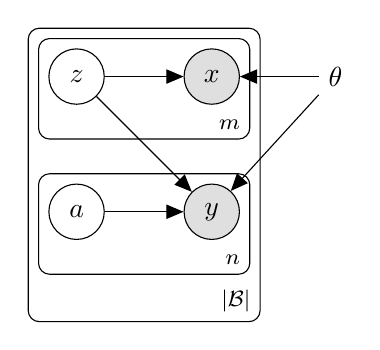
\begin{tikzpicture}
\node[obs]	                   (x)		{$ x $};
\node[obs, below = of x]	       (y)		{$ y $};
\node[latent, left = of x]		(z)		{$ z $};
\node[latent, left = of y]		(a)		{$ a $};
\node[right = of x] (theta) {$\theta$};

% Connect nodes
\edge{a}{y};
\edge{z}{x};
\edge{z}{y};
\edge{theta}{y,x};

% add plates
\plate {L1-sentence} {(x)(z)} {$ m $};
\plate {L2-sentence} {(y)(a)} {$ n $};
\plate {corpus} {(L1-sentence) (L2-sentence)} {$|\mathcal B|$};

\end{tikzpicture}
%\caption{\label{fig:GM2}This model is a refinement of that in \rfig{GM1}, where the latent variable $z$ that participates in generating the aligned sentences. This allows for representations to be ``disambiguated'' in context.}
%\end{figure}
	}
	\end{textblock*}
	
	\begin{textblock*}{\textwidth}(0.32\textwidth,0.35\textheight)
	\begin{figure}
    \begin{overprint}
    \onslide<1>\includegraphics[scale=0.2]{animation/embed1}
    \onslide<2>\includegraphics[scale=0.2]{animation/embed2}
    \onslide<3>\includegraphics[scale=0.2]{animation/embed3}
    \onslide<4>\includegraphics[scale=0.2]{animation/embed4}
    \onslide<5>\includegraphics[scale=0.2]{animation/embed5}
    \onslide<6>\includegraphics[scale=0.2]{animation/embed6}
    \onslide<7>\includegraphics[scale=0.2]{animation/embed7}
    \onslide<8>\includegraphics[scale=0.2]{animation/embed8}
    \onslide<9->\includegraphics[scale=0.2]{animation/embed9} 
    \end{overprint}
\end{figure}
	%\includegraphics[scale=0.2]{animation/embed1}
	%\includegraphics[scale=0.2]{animation/embed2} \pause
	%\includegraphics[scale=0.2]{animation/embed3} \pause
	%\includegraphics[scale=0.2]{animation/embed4} \pause
	%\includegraphics[scale=0.2]{animation/embed5} \pause
	%\includegraphics[scale=0.2]{animation/embed6} \pause
	%\includegraphics[scale=0.2]{animation/embed7} \pause
	%\includegraphics[scale=0.2]{animation/embed8} \pause
	%\includegraphics[scale=0.2]{animation/embed9} \pause
	
	%\begin{small}
	%		\begin{tabular}{p{0.5cm} | p{1.5cm} p{1.5cm} p{1.5cm} p{1.5cm}}
	%		\only<3->{$X$ & \textcolor{blue}{quickly$_1$} & \textcolor{blue}{evacuate$_2$} & \textcolor{blue}{the$_3$} & \textcolor{blue}{area$_4$}} \\
	%		\only<3->{& $\uparrow$ & $\uparrow$ & $\uparrow$ & $\uparrow$} \\
	%		\only<2->{$Z$ & $z_{\textcolor{blue}{1}}$ & $z_{\textcolor{blue}{2}}$ & $z_{\textcolor{blue}{3}}$ & $z_{\textcolor{blue}{4}}$} \\
	%		& & & & \\
	%		\only<4->{$A$ & $a_{\textcolor{orange!90!yellow}{1}}=\textcolor{blue}{2}$ & $a_{\textcolor{orange!90!yellow}{2}}=\textcolor{blue}{3}$ & $a_{\textcolor{orange!90!yellow}{3}}=\textcolor{blue}{4}$ & $a_{\textcolor{orange!90!yellow}{4}}=\textcolor{blue}{1}$ }\\
	%		\only<5->{$Z_a$ & $z_{\textcolor{blue}{2}}$ & $z_{\textcolor{blue}{3}}$ & $z_{\textcolor{blue}{4}}$ & $z_{\textcolor{blue}{1}}$} \\
	%		 \only<6->{& $\downarrow$ & $\downarrow$ & $\downarrow$ & $\downarrow$ } \\
	%		\only<6->{$Y$ & \textcolor{orange!90!yellow}{deje$_1$} & \textcolor{orange!90!yellow}{el$_2$} & \textcolor{orange!90!yellow}{lugar$_3$} & \textcolor{orange!90!yellow}{r\'{a}pidamente$_4$}} \\
		%	\end{tabular}
	%\end{small}
	\end{textblock*}
	
	%\begin{textblock*}{\textwidth}(0.1\textwidth,0.9\textheight)
	%Marginalising alignments collects additional training data for $z$
	%\end{textblock*}


}


\frame[<+->]{ \frametitle{Learning}
\only<2->{
\begin{textblock*}{0.31\textwidth}(0.73\textwidth,0.2\textheight)
		\begin{center}
		\includegraphics[scale=0.44]{meanstd}\\	
		\hfill\textcolor{blue}{\begin{footnotesize}
		evacuate$_1$ the$_2$ area$_3$
		\end{footnotesize}}
		\end{center}
		\end{textblock*}
}
\only<5->{		
\begin{textblock*}{0.31\textwidth}(0.73\textwidth,0.55\textheight)
		\begin{center}
		\includegraphics[scale=0.33]{decxy.png}
		\end{center}
		\end{textblock*}
}

	\begin{textblock*}{\textwidth}(0.07\textwidth,0.3\textheight)
	\begin{enumerate} \small
		\item Read sentence
		\item Predict posterior mean $\mu_i$ and std $\sigma_i$
		%\begin{columns}
		%\begin{column}{0.4\textwidth}
		%\includegraphics[scale=0.4]{img/meanstd}
		%\end{column}
		%\begin{column}{0.4\textwidth}
		%\hfill\textcolor{blue}{Evacuate$_1$ the$_2$ area$_3$}
		%\end{column}
		%\end{columns}
		\item Sample $z_i \sim \mathcal N(\mu_i, \sigma^2_i)$
		%$z_i = \mu_i + \sigma_i \epsilon_i$ \\
		%where $\epsilon_i \sim \mathcal N(0,I)$ 
		\vspace{1cm}
		\item Predict categorical distributions
		\item Generate observations \\ %by marginalising latent alignments\\
		\textcolor{blue}{evacuate$_1$ the$_2$ area$_3$} ~/~ \textcolor{orange!90!yellow}{deje$_1$ el$_2$ lugar$_3$} \\
		
		%\begin{itemize}
		%	\item $P_\theta(x_1^m|z_1^m) = \prod_{i=1}^m P_\theta(X=x_i|z_i)$
		%	\item $P_\theta(y_1^m|x_1^m, z_1^m) = \prod_{j=1}^n \sum_{a_j=1}^m P(a_j|m) P_\theta(Y=y_j|z_i)$
		%\end{itemize}
		\vspace{0.3cm}
		\item Maximise a lowerbound on likelihood\\
		\textcolor{gray}{(Kingma and Welling, 2014)}
	\end{enumerate}		
	\end{textblock*}
\only<6->{	
	\begin{textblock*}{0.31\textwidth}(0.2\textwidth,0.91\textheight)
		\begin{center}
		\includegraphics[scale=0.28]{elbo.png}
		\end{center}
		\end{textblock*}
}	
}

\begin{comment}
\frame[<+->]{ \frametitle{The softmax problem}
Categorical parameters are expensive to compute 
\begin{equation*}
\begin{aligned}
X &\sim \Cat(\mathbf f)\\
\mathbf f &= \softmax (\hat{\mathbf f}) \\
f_{x} &= \frac{\exp(\hat f_x)}{\sum_{x' \in \mathcal X} \exp(\hat f_{x'})}
\end{aligned}
\end{equation*}

\pause

\begin{itemize}
	\item $\mathbf f_1^m$ requires normalising $m$ distributions over the vocabulary of L$_1$, thus it takes time $O(m \times v_1)$
	\item $\mathbf g_1^m$ requires normalising $m$ distributions over the vocabulary of L$_2$, thus it takes time $O(m \times v_2)$
\end{itemize}

\ack{$v_1 = |\mathcal X|$ is the size of the vocabulary of $L_1$; $v_2 = |\mathcal Y|$ is the size of the vocabulary of $L_2$}

}

\frame[<+->]{ \frametitle{Efficient softmax}
Logistic regression
\begin{equation*}
p(x|z) = \frac{\exp(s(z, x))}{\sum_{x'\in \mathcal X} \exp(s(z, x'))}
\end{equation*}

\pause

Define
\begin{itemize}
	\item a set $\mathcal C(x)$ such that $x \in \mathcal C$
	\item a set $\mathcal N(x)$ such that $\mathcal C(x) \cap \mathcal N(x) = \emptyset$
\end{itemize}

\pause 
Re-express normaliser for $p(x|z)$ 
\begin{equation*}
\sum_{x'\in \mathcal X} \exp(s(z, x')) = \sum_{x'\in \mathcal C(x)} \exp(s(z, x')) + \sum_{x'\in \mathcal N(x)} \kappa(x')\exp(s(z, x'))
\end{equation*}
\begin{itemize}
	\item $\kappa(x') = \frac{1}{q(x')}$ and $q(x')$ is an importance distribution
\end{itemize}

}

\frame[<+->]{ \frametitle{Approximate $p(x|z)$}

Logistic regression
\begin{equation*}
p_\theta(x|z) = \frac{\exp(s_\theta(z, x))}{\sum_{x'\in \mathcal X} \exp(s_\theta(z, x'))}
\end{equation*}

\pause

Build
\begin{itemize}
	\item a set $\mathcal C$ containing all L$_1$ words in batch
	\item a set $\mathcal N$ sampling uniformly without replacement from $\mathcal X \setminus \mathcal C$
\end{itemize}

\pause 
Approximate normaliser for $p_\theta(x|z)$
\begin{equation*}
\sum_{x'\in \mathcal X} \exp(s_\theta(z, x')) \approx \sum_{x'\in \mathcal C} \exp(s_\theta(z, x')) + \sum_{x'\in \mathcal N} \frac{|\mathcal X \setminus \mathcal C|}{|\mathcal N|}\exp(s_\theta(z, x'))
\end{equation*}
\begin{itemize}
	\item $s_\theta(z, x) = z^\top \mathbf c_x + b_x$ \\
	$\mathbf c_x = \text{lookup}_\theta(x)$ is a deterministic embedding, $b_x$ a bias term
\end{itemize}

}

\frame[<+->]{ \frametitle{Approximate $p(y|z)$}

Logistic regression
\begin{equation*}
p_\theta(y|z) = \frac{\exp(u_\theta(z, y))}{\sum_{y'\in \mathcal Y} \exp(u_\theta(z, y'))}
\end{equation*}

\pause

Build
\begin{itemize}
	\item a set $\mathcal C$ containing all L$_2$ words in batch
	\item a set $\mathcal N$ sampling uniformly without replacement from $\mathcal Y \setminus \mathcal C$
\end{itemize}

\pause 
Approximate normaliser for $p_\theta(y|z)$
\begin{equation*}
\sum_{y'\in \mathcal X} \exp(s_\theta(z, y')) \approx \sum_{y'\in \mathcal C} \exp(s_\theta(z, y')) + \sum_{y'\in \mathcal N} \frac{|\mathcal Y \setminus \mathcal C|}{|\mathcal N|}\exp(s_\theta(z, y'))
\end{equation*}
\begin{itemize}
	\item $s_\theta(z, y) = z^\top \mathbf c_y + b_y$ \\
	$\mathbf c_y = \text{lookup}_\theta(y)$ is a deterministic embedding, $b_y$ a bias term
\end{itemize}

}

\frame[<+->]{ \frametitle{Complementary Sum Sampling (CSS) - Summary}
The approximation effectively reduces the size of the support of the categorical variable
\begin{itemize}
	\item in each batch, the support is made of the word types in the batch
	\item along with a random subset of ``negative words''
	\item this is similar to ``negative sampling'' but improves on asymptotic behaviour
	\item it only affects the softmax: the model remains generative
\end{itemize}

\ack{\citep{pmlr-v54-botev17a}}
}

\end{comment}

\subsection{Evaluation}

\frame{ \frametitle{Data}

\begin{tabular}{l r r}
\toprule
Corpus     & Sentence pairs (million) & Tokens (million)\\ \midrule
Europarl \textsc{En-Fr} & $1.7$  & $42.5$ \\ %1,768,554  & 42548586/44975891\\
Europarl \textsc{En-De} & $1.7$  & $43.5$ \\ %1,756,152  & 43485348/39832101\\
%Giga \textsc{En-Fr}     & $18.3$ & $419.6$ \\ \bottomrule %  18,302,058 & 419688707/482622626\\
 \bottomrule
\end{tabular}
}

\frame[<+->]{ \frametitle{Architecture}
%\begin{textblock*}{0.35\textwidth}(0.8\textwidth,0.05\textheight)

\begin{figure}
  \includegraphics[width=0.42\textwidth]{architecture.pdf}
 %  \hfill
%   \includegraphics[width=0.42\textwidth]{dec.png}
\end{figure}


%\end{textblock*}

%\begin{textblock*}{\textwidth}(0.05\textwidth,0.15\textheight)
%\begin{itemize}
%\item Embedding 128d
%\item BiLSTM 128d
%\item Z 100d
%\end{itemize}
%\end{textblock*}
}

\frame[<+->, fragile]{\frametitle{Word Alignment}
\scalebox{0.85}{
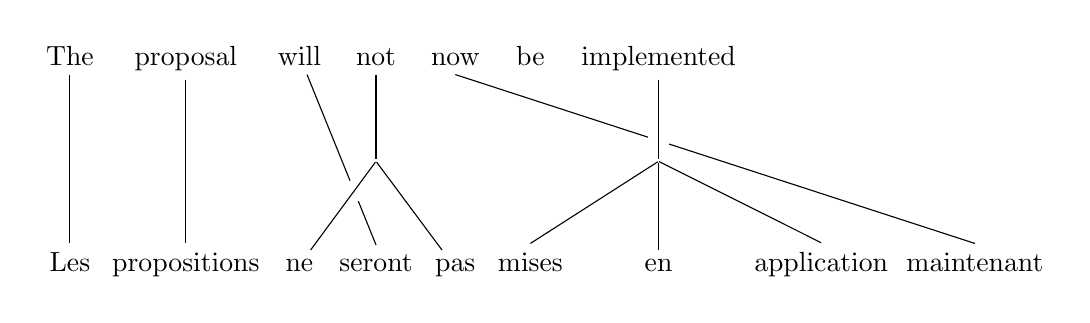
\begin{tikzpicture}[ampersand replacement=\&]
% First make a matrix containing as many columns as the longest sentence.
% Each cell contains a node whose label is identical to the word itself
\matrix[column sep=0em,row sep=.4in] {
% First sentence
\hnode{The} \& \hnode{proposal} \& \hnode{will} \& \hnode{not} \& \hnode{now} \& \hnode{be} \&  \hnode{implemented}  \&\\
% Now create some dummy nodes to make intermediate nodes
\& \& \& \node[inner sep={0pt},minimum width=0pt] (p1) {}; \& \& \& \node[inner sep={0pt},minimum width=0pt] (p2) {};\\
% Second sentence
\hnode{Les} \& \hnode{propositions} \& \hnode{ne}  \& \hnode{seront} \& \hnode{pas} \& \hnode{mises} \& \hnode{en} \& \hnode{application} \& \hnode{maintenant}\\
};
% Now connect the nodes.  For paths that we want to break, name the path
\draw (The) -- (Les);
\draw (proposal) -- (propositions);
\draw[name path=willP] (will) -- (seront.north);
\draw (not) -- (p1);
\path[name path=neP] (p1) -- (ne);
\draw (p1) -- (pas);
\draw[name path=nowP] (now.south)  -- (maintenant.north);
\path[name path=impP] (implemented) -- (p2);
\draw (p2) -- (mises.north);
\draw (p2) -- (en);
\draw (p2) -- (application.north);
% Now break the paths at the intersection by drawing a white circle over it
\fill[white, name intersections={of=willP and neP}] (intersection-1) circle (4pt);
\fill[white, name intersections={of=nowP and impP}] (intersection-1) circle (4pt);
% Finally redraw the path you don't want broken
% Is there a more elegant way to do this?
\draw (p1) -- (ne);
\draw (implemented) -- (p2);
\end{tikzpicture}
}
}

\frame{ \frametitle{Word Alignment}
\begin{itemize}
\item Model \textcolor{blue}{selection} on Dev set %Handsards
%\item Test set Handsards
\end{itemize}

\center
\begin{tabular}{l c c}
      & AER  $\downarrow$  &   \\
\toprule
Model       & En-Fr  & En-De  \\ \midrule
\textsc{IBM1}  & 32.45 & 46.71 \\  
\textsc{IBM2}  & 22.61 &  40.11 \\  
\textsc{EmbAlign} & $ 29.43\pm1.84$ & $48.09\pm2.12$ \\ \bottomrule
\end{tabular}

}

\frame[<+->]{ \frametitle{Lexical Substitution}
\only<1->{
\begin{textblock*}{0.3\textwidth}(0.1\textwidth,0.32\textheight)
		\includegraphics[scale=0.42]{lexsuba.png}\\	
		
\end{textblock*}
}
\only<2->{
\begin{textblock*}{0.1\textwidth}(0.4\textwidth,0.24\textheight)
		\includegraphics[scale=0.30]{lexsubb.png}\\	
		
\end{textblock*}
}
\only<3->{
\begin{textblock*}{0.1\textwidth}(0.4\textwidth,0.96\textheight)
		\includegraphics[scale=0.30]{lexsubc.png}\\	
		
\end{textblock*}
}
}


\frame[<+->]{ \frametitle{Lexical Substitution}

%\center
\begin{tabular}{l c c }
%& GAP $\uparrow$ &  & \\
\toprule
Model                                                           & GAP $\uparrow$ & \begin{footnotesize}
Training size
\end{footnotesize}\\ \midrule
%\begin{tabular}[c]{@{}c@{}}Melamud et al.\\ 2015\end{tabular}	& 44.9         \\
%\begin{tabular}[c]{@{}c@{}}Melamud et al.\\ 2016\end{tabular} & 56.1         \\
\textsc{Random}   & $30.0$ & \\
\textsc{SkipGram} \\ \begin{footnotesize} \textcolor{gray}{(Melamud et al., 2015)}\end{footnotesize} & $44.9$  & ukWaC-2B \\ 
\textsc{BSG} \\ \begin{footnotesize} \textcolor{gray}{(Bražinskas et al., 2017)} \end{footnotesize}     &  $ 46.1$ & ukWaC-2B \\ \hline

\textsc{En} & $21.31\pm1.05$  & \\ \hline

\textsc{En-Fr} & $42.19\pm0.57$ & Euro-42M \\
\textsc{En-De} & $42.07\pm0.47$  & \\ \bottomrule
\end{tabular}

}

\frame[<+->]{ \frametitle{Sentence Evaluation (SentEval)}
\only<1->{
\begin{textblock*}{\textwidth}(0.1\textwidth,0.25\textheight)
		\includegraphics[scale=0.29]{senteval.png}\\	
		
\end{textblock*}
}
\only<2->{
\begin{textblock*}{\textwidth}(0.55\textwidth,0.05\textheight)
		\includegraphics[scale=0.28]{embedalign.png}\\	
		
\end{textblock*}
}
\only<3->{
\begin{textblock*}{\textwidth}(0.35\textwidth,0.74\textheight)
		\includegraphics[scale=0.25]{w2vecSenteval.png}\\	
		
\end{textblock*}
}
}

\frame[<+->]{ \frametitle{Sentence Evaluation (SentEval)}

\scalebox{0.615}{
\begin{tabular}{lcccccccccc}

 &     &    &   &   &   & ACC $\uparrow$ &    ACC/F1 $\uparrow$     & CORR $\uparrow$ &  &   CORR $\uparrow$   \\
\toprule
Model    & MR    & CR    & SUBJ  & MPQA  & SST  & TREC & MRPC        & SICK-R & SICK-E & STS14     \\ \midrule
\textsc{SkipGram}$_{\text{En}}$    & \textbf{70.96} & \textbf{76.16}  & \textbf{87.24}  & \textbf{86.87}  & \textbf{73.64} & 65.20 & 70.7/80.1   & 0.710  &  76.2 & 0.45/0.49 \\

\midrule
\textsc{En}   & 57.5  & 67.1  & 72.0    & 70.8  & 57.0   & 58.0   & 70.6/80.3   & 0.648  & 74.4   & 0.59/0.59 \\
\textsc{En-Fr}    & 64.0 & 71.8  & 79.1  & 81.5  & 64.7 & 58.4 & 72.1/81.2   & 0.682  & 74.6   & 0.60/0.59 \\
\textsc{En-De}    & 62.6  & 68.0    & 77.3 & 82.0    & 65.0   & 66.8 & 70.4/79.8   & 0.681  & 75.5  & 0.58/0.58 \\
\textsc{Combo} & 66.1  & 72.4 & 82.4 & 84.4 & 69.8 & \textbf{69.0}   & \textbf{71.9}/\textbf{80.6} & \textbf{0.727} & \textbf{76.3}  & \textbf{0.62}/\textbf{0.61} \\ \bottomrule

\end{tabular}
}
}

\frame[<+->]{ \frametitle{Sentence Evaluation (SentEval)}


\scalebox{0.585}{
\begin{tabular}{lcccccccccc}

 &     &    &   &   &   & ACC $\uparrow$ &    ACC/F1 $\uparrow$     & CORR $\uparrow$ &  &   CORR $\uparrow$   \\
\toprule
Model    & MR    & CR    & SUBJ  & MPQA  & SST  & TREC & MRPC        & SICK-R & SICK-E & STS14     \\ \midrule
\textsc{SkipGram}$_{\text{En}}$    & \textbf{70.96} & \textbf{76.16}  & \textbf{87.24}  & \textbf{86.87}  & \textbf{73.64} & 65.20 & 70.7/80.1   & 0.710  &  76.2 & 0.45/0.49 \\

\midrule
\textsc{En}   & 57.5  & 67.1  & 72.0    & 70.8  & 57.0   & 58.0   & 70.6/80.3   & 0.648  & 74.4   & 0.59/0.59 \\
\textsc{En-Fr}    & 64.0 & 71.8  & 79.1  & 81.5  & 64.7 & 58.4 & 72.1/81.2   & 0.682  & 74.6   & 0.60/0.59 \\
\textsc{En-De}    & 62.6  & 68.0    & 77.3 & 82.0    & 65.0   & 66.8 & 70.4/79.8   & 0.681  & 75.5  & 0.58/0.58 \\
\textsc{Combo} & 66.1  & 72.4 & 82.4 & 84.4 & 69.8 & \textbf{69.0}   & \textbf{71.9}/\textbf{80.6} & \textbf{0.727} & \textbf{76.3}  & \textbf{0.62}/\textbf{0.61} \\ 
\midrule
 &     &    &   &   &   & &    &  &  &     \\
  &     &    &   &   &   &  &    & &  &    \\
\midrule
\textsc{SkipGram} \\ \begin{footnotesize}
\textcolor{gray}{(Conneau et al., 2017)}
\end{footnotesize} & \textbf{77.7}  & \textbf{79.8}  & \textbf{90.9}  & \textbf{88.3}  & \textbf{79.7} & \textbf{83.6} & \textbf{72.5}/\textbf{81.4}   & \textbf{0.803}  & \textbf{78.7}   & \textbf{0.65}/\textbf{0.64} \\
\textsc{nmt}$_{\text{En-Fr}}$ \\ \begin{footnotesize}
\textcolor{gray}{(Conneau et al., 2017)}
\end{footnotesize} &  64.7 & 70.1  & 84.8  & 81.5  & - & 82.8  &  - & -  & -   & 0.42/0.43 \\
  \bottomrule
\end{tabular}
}


}



%\frame[<+->]{ \frametitle{Word Similarity}
%\begin{itemize}
%\item[synonym] 
%\begin{itemize}
%\item cup - mug
%\item glasses - spectacles 
%\end{itemize}
%\item[similar]
%\begin{itemize}
%\item alligator - crocodile
%\item love - affection 
%\end{itemize}
%\item[related]
%\begin{itemize}
%\item car - tyre
%\item car - motorway 
%\end{itemize}

%\end{itemize}
%}



\subsection{Conclusions and Future Work}
\frame[<+->]{ \frametitle{Conclusions}
\begin{itemize}
%\item what we did
%\item We will modify \textcolor{blue}{alignment} distribution 
%\item We will extend the  \textcolor{blue}{hierarchy} of the model
%\item We will expand the  distributional context to \textcolor{blue}{multiple foreign languages} at once \\
%This will increase the model \textcolor{blue}{disambiguation} power 
\item Generative training 

\begin{itemize}
\item model learns form positive examples 
\item no need for context window 
\end{itemize}

\item Translation data 
\begin{itemize}
\item less ambiguous embeddings
\item model helps with semantic tasks e.g.  \textcolor{blue}{paraphrasing}
\end{itemize}

\end{itemize}
}





\frame[<+->]{ \frametitle{Open Source Code}
\begin{itemize}
\item Try pre-trained Europarl model on SentEval: \\
\url{https://github.com/uva-slpl/embedalign/blob/master/notebooks/senteval_embedalign.ipynb}


\end{itemize}
}

\begin{comment}
\section{Bayesian Skip-Gram}

\frame[<+->]{ \frametitle{Bayesian Skip-Gram}


\begin{columns}
\begin{column}{0.45\textwidth}
\includegraphics[scale=0.35]{bsg-example}
\end{column}
\quad
\begin{column}{0.45\textwidth}
\begin{footnotesize}
\only<1>{
\emph{``Representing a word as a distribution provides many potential benefits. For example, such embeddings let us encode generality of terms (e.g., `kakapo' is a type of `bird'), characterize uncertainty about semantic properties of the corresponding referent (e.g., a proper noun, such as `John', encodes little about the person it refers to) or represent polysemy (e.g., `kiwi' may refer to a fruit, a bird or a New Zealander).''}
}
\only<2>{
\emph{``In principle, using densities to represent words provides a natural way of encoding entailment: the decision regarding entailment relation can be made by testing the level sets of the distributions for `soft inclusion'. For example, in Figure 1, the ellipse for `kakapo' lies within the ellipse for `bird'. ''}
}
\end{footnotesize}
\end{column}

\end{columns}


%\ack{\citet{bravzinskas2017embedding}}
}


\frame[<+->]{ \frametitle{Model}
Generative model: for $i=1, \ldots, m$\\

\begin{equation*}
\begin{aligned}
Z_i|x_i &\sim \mathcal N(\boldsymbol \mu_{x_i}, \diag(\boldsymbol \sigma_{x_i} \odot \boldsymbol \sigma_{x_i}))\\
\boldsymbol \mu_{x_i} &= \text{lookup}_\theta(x_i)\\
\boldsymbol \sigma_{x_i} &= \softplus(\text{lookup}_\theta(x_i))
\end{aligned}
\end{equation*}
\pause
~for $k \in \mathcal K_i = \{\underbrace{i-n, \ldots, i-1,  i+1, \ldots, i+n}_{n \text{ words on each side of }x_i}\}$ \pause
\begin{equation*}
\begin{aligned}
X_k|z_i &\sim \Cat(\mathbf f_i) \\ 
\mathbf f_i &= \softmax(\affine_\theta(z_i))
\end{aligned}
\end{equation*}

\pause

Inference model
\begin{equation*}
\begin{aligned}
Z_i|x_{i-n}^{i+n} &\sim \mathcal N(\mathbf u_i, \diag(\mathbf s_i \odot \mathbf s_i))\\
\mathbf h_i &= \sum_{k \in \mathcal K_i} \relu(\affine_\lambda([x_k, x_i])) \\
\mathbf u_i &= \affine_\lambda(h_i) \\
\mathbf s_i &= \softplus(\affine_\lambda(h_i)) 
\end{aligned}
\end{equation*}


}

\frame[<+->]{ \frametitle{ELBO}
\begin{equation*}
\begin{aligned}
\mathbb E_{q_\lambda(z_1^m|x_1^m)} \left[ \log \alert{\prod_{i=1}^m \prod_{k \in \mathcal K_i} P(x_k|z_i)} \right] - \KL{q_\lambda(z_1^m|x_1^m)}{p_\theta(z_1^m|x_1^m)}
\end{aligned}
\end{equation*}
\begin{itemize}
	\item observation model is trained discriminatively\\
	latent variables generate overlapping subsets of observations
\end{itemize}

}

\frame[<+->]{ \frametitle{ELBO - KL term}
\begin{equation*}
\begin{aligned}
\mathbb E_{q_\lambda(z_1^m|x_1^m)} \left[ \log \prod_{i=1}^m \prod_{k \in \mathcal K_i} P_\theta(x_k|z_i) \right] - \textcolor{blue}{\KL{q_\lambda(z_1^m|x_1^m)}{p_\theta(z_1^m|x_1^m)}}
\end{aligned}
\end{equation*}

KL term
\begin{equation*}
\begin{aligned}
&\textcolor{blue}{\KL{q_\lambda(z_1^m|x_1^m)}{p_\theta(z_1^m|x_1^m)}} \\ \pause
 &=  \sum_{i=1}^m \KL{q_\lambda(z_i|x_{i-n}^{i+n})}{p_\theta(z_i|x_i)} \\ \pause
 &=  \sum_{i=1}^m \KL{\underbrace{\mathcal N(\mathbf u_i, \diag(\mathbf s_i \odot \mathbf s_i))}_{\text{inference model}}}{\underbrace{\mathcal N(\boldsymbol \mu_{x_i}, \diag(\boldsymbol \sigma_{x_i} \odot \boldsymbol \sigma_{x_i}))}_{\text{prior}}} 
\end{aligned}
\end{equation*}

\ack{Empirical Bayes: point estimate prior parameters}

}


\begin{frame}{ELBO - Likelihood term}
\begin{equation*}
\begin{aligned}
\textcolor{blue}{\mathbb E_{q_\lambda(z_1^m|x_1^m)} \left[ \log \prod_{i=1}^m \prod_{k \in \mathcal K_i} P_\theta(x_k|z_i) \right]} - \KL{q_\lambda(z_1^m|x_1^m)}{p_\theta(z_1^m|x_1^m)}
\end{aligned}
\end{equation*}
\pause

Likelihood term
\begin{small}
\begin{equation*}
\begin{aligned}
\textcolor{blue}{\mathbb E_{q_\lambda(z_1^m|x_1^m)} \left[ \log \prod_{i=1}^m \prod_{k \in \mathcal K_i} P_\theta(x_k|z_i) \right]}  \pause
 &= \mathbb E_{q_\lambda(z_1^m|x_1^m)} \left[  \sum_{i=1}^m \sum_{k \in \mathcal K_i} \log P_\theta(x_k|z_i) \right] \\ \pause
&= \sum_{i=1}^m \sum_{k \in \mathcal K_i} \mathbb E_{q_\lambda(z_i|x_{i-n}^{i+n})} \left[  \log P_\theta(x_k|z_i) \right] \\ \pause
&= \sum_{i=1}^m \sum_{k \in \mathcal K_i} \mathbb E_{q_\lambda(z_i|x_{i-n}^{i+n})} \left[  \log \Cat(x_k|\mathbf f_i) \right]
\end{aligned}
\end{equation*}
\end{small}

\end{frame}

\frame[<+->]{ \frametitle{The softmax problem}

To circumvent an expensive softmax, change the likelihood term
\begin{equation*}
P_\theta(x|z) = \frac{u_\theta(z, x)}{\alert{\sum_{x' \in \mathcal X} u_\theta(z, x')}} \qquad \text{with } u_\theta(\cdot, \cdot) > 0
\end{equation*}
\pause
and re-write the likelihood term
\begin{equation*}
\begin{aligned}
\mathbb E_{q_\lambda(z)} \left[  \log P_\theta(x|z) \right] 
 &= \mathbb E_{q_\lambda(z)} \left[  \log u_\theta(z, x) - \log \alert{\sum_{x'\in \mathcal X}u_\theta(z, x')}\right] \\ \pause
 &=\mathbb E_{q_\lambda(z)} \left[  \log u_\theta(z, x) \right] - \mathbb E_{q_\lambda(z)} \left[ \log \alert{\sum_{x'\in \mathcal X}u_\theta(z, x')}\right]
\end{aligned}
\end{equation*}


}

\frame[<+->]{ \frametitle{Lowerbound on likelihood term}
Then (by design) let
\begin{equation*}
u_\theta(z, x) = \underbrace{P(x)}_{\text{fixed}}\mathcal N(z|\boldsymbol \mu_x, \diag(\boldsymbol \sigma_x \odot \boldsymbol \sigma_x))
\end{equation*}
\pause

And bound $ \mathbb E_{q_\lambda(z)} \left[ \log \alert{\sum_{x'\in \mathcal X}u_\theta(z, x')}\right] $ \pause
\begin{equation*}
\begin{aligned} 
&=\mathbb E_{q_\lambda(z)} \left[ \log \alert{\sum_{x'\in \mathcal X} P(x)\mathcal N(z|\boldsymbol \mu_x, \diag(\boldsymbol \sigma_x \odot \boldsymbol \sigma_x))} \right] \\ \pause
&=\mathbb E_{q_\lambda(z)} \left[ \log \alert{\mathbb E_{P(x)}\left[ \mathcal N(z|\boldsymbol \mu_x, \diag(\boldsymbol \sigma_x \odot \boldsymbol \sigma_x)) \right]} \right] \\ \pause
&\overset{\text{JI}}{\ge} \mathbb E_{q_\lambda(z)} \left[ \textcolor{blue}{\mathbb E_{P(x)}\left[ \log \mathcal N(z|\boldsymbol \mu_x, \diag(\boldsymbol \sigma_x \odot \boldsymbol \sigma_x)) \right]} \right]
\end{aligned}
\end{equation*}
\pause

\begin{itemize}
	\item $P(x)$ does not depend on $\theta$, we can compute an MC estimate\\
	e.g. empirical (unigram) distribution
\end{itemize}

}

\end{comment}



\section{EmbedAlign-2}

\frame[<+->]{ \frametitle{EmbedAlign-2}
\begin{itemize}

\item Hierarchical generative model of words and sentences by exploiting automatically generated paraphrasing data.
\item Model embeds sentences and words as probability densities.
\item Model learns from sentence-aligned corpora by marginalisation of
latent lexical alignments.
\item Testing on different sentence representation benchmarks.
\end{itemize}
}


\frame[<+->]{ \frametitle{EmbedAlign-2}
\begin{itemize}

\item Hierarchical generative model of words and sentences by exploiting automatically generated paraphrasing data.
\item Model embeds sentences and words as probability densities.
\item Model learns from sentence-aligned corpora by marginalisation of
latent lexical alignments.
\item Testing on different sentence representation benchmarks.
\end{itemize}
}

\frame[<+->]{ \frametitle{EmbedAlign-2}
\begin{itemize}
\item Wieting and Gimpel (2017) port the pivoting approach in (Bannard and Callison-Burch, 2005) for paraphrasing to NMT. \\ \textit{Paraphrase English sentences by translating to a foreign language and back to English}. 

\item How to represent paraphrases that introduce \red{syntactic variations}.
\item How to represent \red{noisy} automatically generated data. 
\begin{figure}
	\includegraphics[scale=0.33]{para_eg}
	
	\end{figure}

\end{itemize}
}

\frame[<+->]{ \frametitle{EmbedAlign-2}
\begin{itemize}
    \item Parallel data $\langle x_1^m, y_1^n \rangle$ where $x_1^m$ is a sentence in original English and $y_1^n$ is a sentence paraphrase English.
    
    \item Hierarchical generative model parameterised by neural networks.


\begin{equation}
\begin{aligned}
S &\sim \mathcal N(0, I)  \label{eq:S} \\
Z_i &\sim \mathcal N(\mu(s), \sigma^2(s)) 
\end{aligned}
\end{equation}

 \scalebox{0.80}{

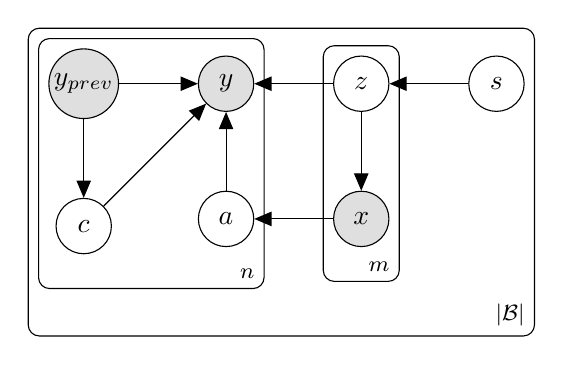
\begin{tikzpicture}
\node[obs]	       (y)		{$ y $};
\node[latent, right = of y]		(z)		{$ z $};
\node[obs, below = of z]	                   (x)		{$ x $};
\node[latent, right = of z]		(s)		{$ s $};
\node[latent, below = of y]		(a)		{$ a $};
\node[obs, left = of y]		(yp)		{$ y_{prev} $};
\node[latent, below = of yp]		(c)		{$ c $};
%\node[right = of x] (theta) {$\theta$};

% Connect nodes
\edge{a}{y};
\edge{x}{a};
\edge{z}{x};
\edge{s}{z};
\edge{z}{y};
\edge{c}{y};
\edge{yp}{c,y};
%\edge{theta}{y,x,z};

% add plates
\plate {L1-sentence} {(x)(z)} {$ m $};
\plate {L2-sentence} {(y)(a)(yp)(c)} {$ n $};
\plate {corpus} {(s) (L1-sentence) (L2-sentence)} {$|\mathcal B|$};
\end{tikzpicture}


}
\end{itemize}





}

\frame[allowframebreaks]{\frametitle{Model}
\begin{itemize}
\item With a Gaussian distributed sentence embedding $s$ and word embeddings $z_1^m$, we can marginalise \cblue{collocation} and \cblue{alignment} components.\\
Latent decision is modelled with a Bernoulli trial: 
\begin{equation}
\begin{aligned}
p(y_j|x_1^m, z_1^m) &= p(c_j=0) p(y_j|y_{j-1}) \\
&+ p(c_j=1) \sum_{a_j=1}^m p(a_j|m, n)p(y_j|z_{a_j}) 
\end{aligned}
\end{equation}

\item Inference: \\
\begin{equation}
q(s, z_1^m) = q_s(s)\prod_{i=1}^m q_{z_i}(z_i)
\end{equation} \\
where $S \sim \mathcal N(\mathbf u_0, \mathbf s_0^2)$ and $Z_i \sim \mathcal N(\mathbf u_i, \mathbf s_i^2)$.

\item \cblue{Collocation} is rudimentary language model condition on previously generated word.
\item \cblue{Alignment} identifying relationships among words in the parallel data.
\item Estimate parameters via maximisation of a lower-bound on marginal likelihood:\\
\begin{equation}
\begin{aligned}\label{eq:objective}
\log p(x_1^m, y_1^n) \ge \mathbb E[\log p(x_1^m|z_1^m)] \\
+ \mathbb E[\log p(y_j|x_1^m,z_1^m)] \\
- \sum_{i=1}^m \mathbb E[ \mathrm{KL}(q(z_i | x) \| p(z| s)) ] \\
- \mathrm{KL}(q(s| x) \| \mathcal N (0, I))
\end{aligned}
\end{equation}


%\item figure of architecture
\end{itemize}
}


\frame{\frametitle{Evaluation}
\begin{itemize}
    \item Sentence-level paraphrases PARANMT-5M with 5 million sentences \blue{EN1-EN2}.
    \item English-French \blue{EN-FR} and English-German \blue{EN-DE} from Europarl-v7.
\end{itemize}
 
\textbf{Word Alignment}
\begin{itemize}
    \item Test alignment error rate (AER) on bilingual models.
    \item report on IBM models 1, 2 and \textsc{FastAlign}.
    
\end{itemize}

\begin{center}
    \scalebox{0.94}{
\begin{tabular}{l c c}
\toprule
Model       & \textsc{En-Fr} $\downarrow$ & \textsc{En-De} $\downarrow$ \\ \midrule
\textsc{IBM1}  & $0.32$ & $0.47$ \\  % .3245 & 0.4671
\textsc{IBM2}  & $0.23$ & $0.40$ \\   % 0.2261 & 0.4011
\textsc{EmbedAlign} & $0.29\pm0.02$ & $0.48 \pm 0.02$ \\
\textsc{FastAlign}  & $0.19$ & $0.36$ \\   \hline
This work & $0.18\pm0.01$ & $0.40\pm0.01$ \\ \bottomrule  % 0.1820 & 0.4013
\end{tabular}
}
\end{center}
}


\frame{\frametitle{Evaluation}
 \scalebox{0.60}{
\begin{tabular}{lcccccccccc}
\toprule
Model    & MR    & CR    & MPQA   & SUBJ  & SST  & TREC & MRPC        & SICK-E & SICK-R & STS14     \\ \midrule
\multicolumn{11}{c}{Baselines}\\ \midrule
\textsc{ELMO} &  79.87 & 84.85  & 89.21 & 94.19  & 85.67 & 92.80 & 72.93/80.90   & 81.21  &  0.82/0.75  & 0.61/0.58 \\ 

\textsc{SkipGram}$_\text{En1}$ & 72.11  & 78.20  & 85.51  & 88.82  & 75.56 & 72.20 & 71.54/81.02   & 76.16  &  0.75/0.66  & 0.44/0.48 \\
 \midrule
 \multicolumn{11}{c}{Ours}\\ \midrule
\textsc{En-Fr}    & 66.76 & 71.18  & 85.40  & 82.32  & 67.52 & 70.45 & 71.90/80.77   & 75.18 &  0.67/0.62  & 0.49/0.50 \\
\textsc{En-De}    & 66.00 & 72.21  & 85.71  & 81.63  & 67.64 & 70.45 & 71.83/80.85   & 75.73 &  0.66/0.62  &  0.49/0.59 \\
\textsc{En1-En2} &  66.88  & 71.59  & 81.80    & 82.97  & 69.14   & 67.30   & 71.33/80.36   & 75.62  & 0.72/0.66   & 0.53/0.52 \\ 
\bottomrule
\end{tabular}
}
}




\frame[<+->]{ \frametitle{EmbedAlign-2}
\begin{itemize}
%\item what we did
%\item We will modify \textcolor{blue}{alignment} distribution 
%\item We will extend the  \textcolor{blue}{hierarchy} of the model
%\item We will expand the  distributional context to \textcolor{blue}{multiple foreign languages} at once \\
%This will increase the model \textcolor{blue}{disambiguation} power 
\item We modify alignment distribution
\begin{itemize}
%\item Generative model of word representation that learns from positive correlations implicitly expressed in translation data
%\item Our model can induce representations useful for downstream  NLP tasks
\item From IBM1 to  \textcolor{blue}{IBM2}  \\ %, fastalign (Dyer et al. 2013)} 
En-Fr 29.43 $\rightarrow$ \textcolor{blue}{18.20} AER
\end{itemize}


\item We model word and sentence embeddings
%Modelling \textcolor{blue}{word} and \textcolor{blue}{sentence level} embeddings 
\begin{itemize}
\item \textbf{M}ovie \textbf{R}eviews 66.10 $\rightarrow$ \textcolor{blue}{70.55} ACC
\item \textbf{M}icrosoft \textbf{P}araphrase 71.90/80.6 $\rightarrow$ \textcolor{blue}{72.93/81.27} ACC/F1
\item \textbf{S}ick \textbf{R} 0.727 $\rightarrow$ \textcolor{blue}{0.770} CORR
\end{itemize}


\item We \textbf{will} expand the  distributional context to \textcolor{blue}{multiple foreign languages} at once

\end{itemize}
}




\section*{References}
	
	%
\frame[plain]{
	\frametitle{Earley intersection}
	
	\begin{footnotesize}
	\begin{align*}
	\textsc{Axioms} & \\
	& \drule{}{\itembrack{S' \ra \bullet S, q, q}}{q \in I} \\
	\textsc{Goal} & \\
	& \itembrack{S' \ra S \bullet, q, r} ~ q \in I \wedge r \in F\\
	\textsc{Scan} & \\
	& \drule{\itembrack{X \ra \alpha \bullet x \beta, q, s}}{\itembrack{X \ra \alpha x \bullet \beta}}{\angbrack{s, x, r} \in E}\\
	\textsc{Predict} & \\
	& \drule{\itembrack{X \ra \alpha \bullet Y \beta, q, r}}{\itembrack{Y \ra \bullet \gamma, r, r}}{Y \ra \gamma \in R} \\
	\textsc{Complete} & \\
	& \drule{\itembrack{X \ra \alpha \bullet Y \beta, q, s}\itembrack{Y \ra \gamma \bullet, s, r}}{\itembrack{X \ra \alpha Y_{s,r} \bullet \beta, q, r}}{X \neq S'} \\
	\textsc{Accept} & \\
	& \drule{\itembrack{S' \ra \bullet S, q, q}\itembrack{S \ra \gamma \bullet, q, r}}{\itembrack{S' \ra  S_{q,r} \bullet, q, r}}{r \in F} 
	\end{align*}
	\end{footnotesize}

	
}




	\frame[allowframebreaks]{ \frametitle{References}
	\cred{TOREAD}: Arthur Brazinskas, Serhii Havrylov, and Ivan Titov. Embedding words as distributions with a bayesian skip-gram model. arXiv preprint arXiv:1711.11027, 2017.
        \bibliographystyle{plainnat}
        \bibliography{BIB}
	}


\end{document}
\grid
